\section*{Introduction}

FAC is the front end part of a compiler which translates programs written in the
F language into a target representation. FAC is written in C using
flex \cite{flex-online} and bison \cite{bison-online}.
It is interesting to note that FAC can potentially support many target
representations.

\subsection*{Architecture}
Fig. \ref{fig:arch-ovw} describes the architecture of FAC.
Its high-level structure is formed by two macro components:
\begin{itemize}
\item Lexer - the lexical analyzer;
\item Parser - which is divided into three parts:
\begin{itemize}
	\item Syntax analysis;
	\item Static semantic analysis;
	\item Target code generation.
\end{itemize}
\end{itemize}

FAC has been written to be modular. Indeed, it is possible to translate any F
program into other representations simply by writing a new printer implementation.
\\
In FAC a printer is a component which takes the three address code (3AC) of an F
program given as input and generates a version of that code translated into a targeted
representation.
\\
Currently, FAC supports three printers:
\begin{itemize}
\item IR (Internal Representation) - useful for educational purposes or to quickly debug the 3AC;
\item C - prints a C program;
\item Java\footnote{for time reasons only the skeleton has been implemented} - prints a Java program.
\end{itemize}

We chose to use two different intermediate representations:
\begin{itemize}
\item Abstract Syntax Three (AST) - because it is easy to perform semantic analysis on this structure;
\item Three Address Code (3AC) - because it is easy to perform code generation by parsing this structure.
\end{itemize}

\begin{figure}[H]
  \centering
  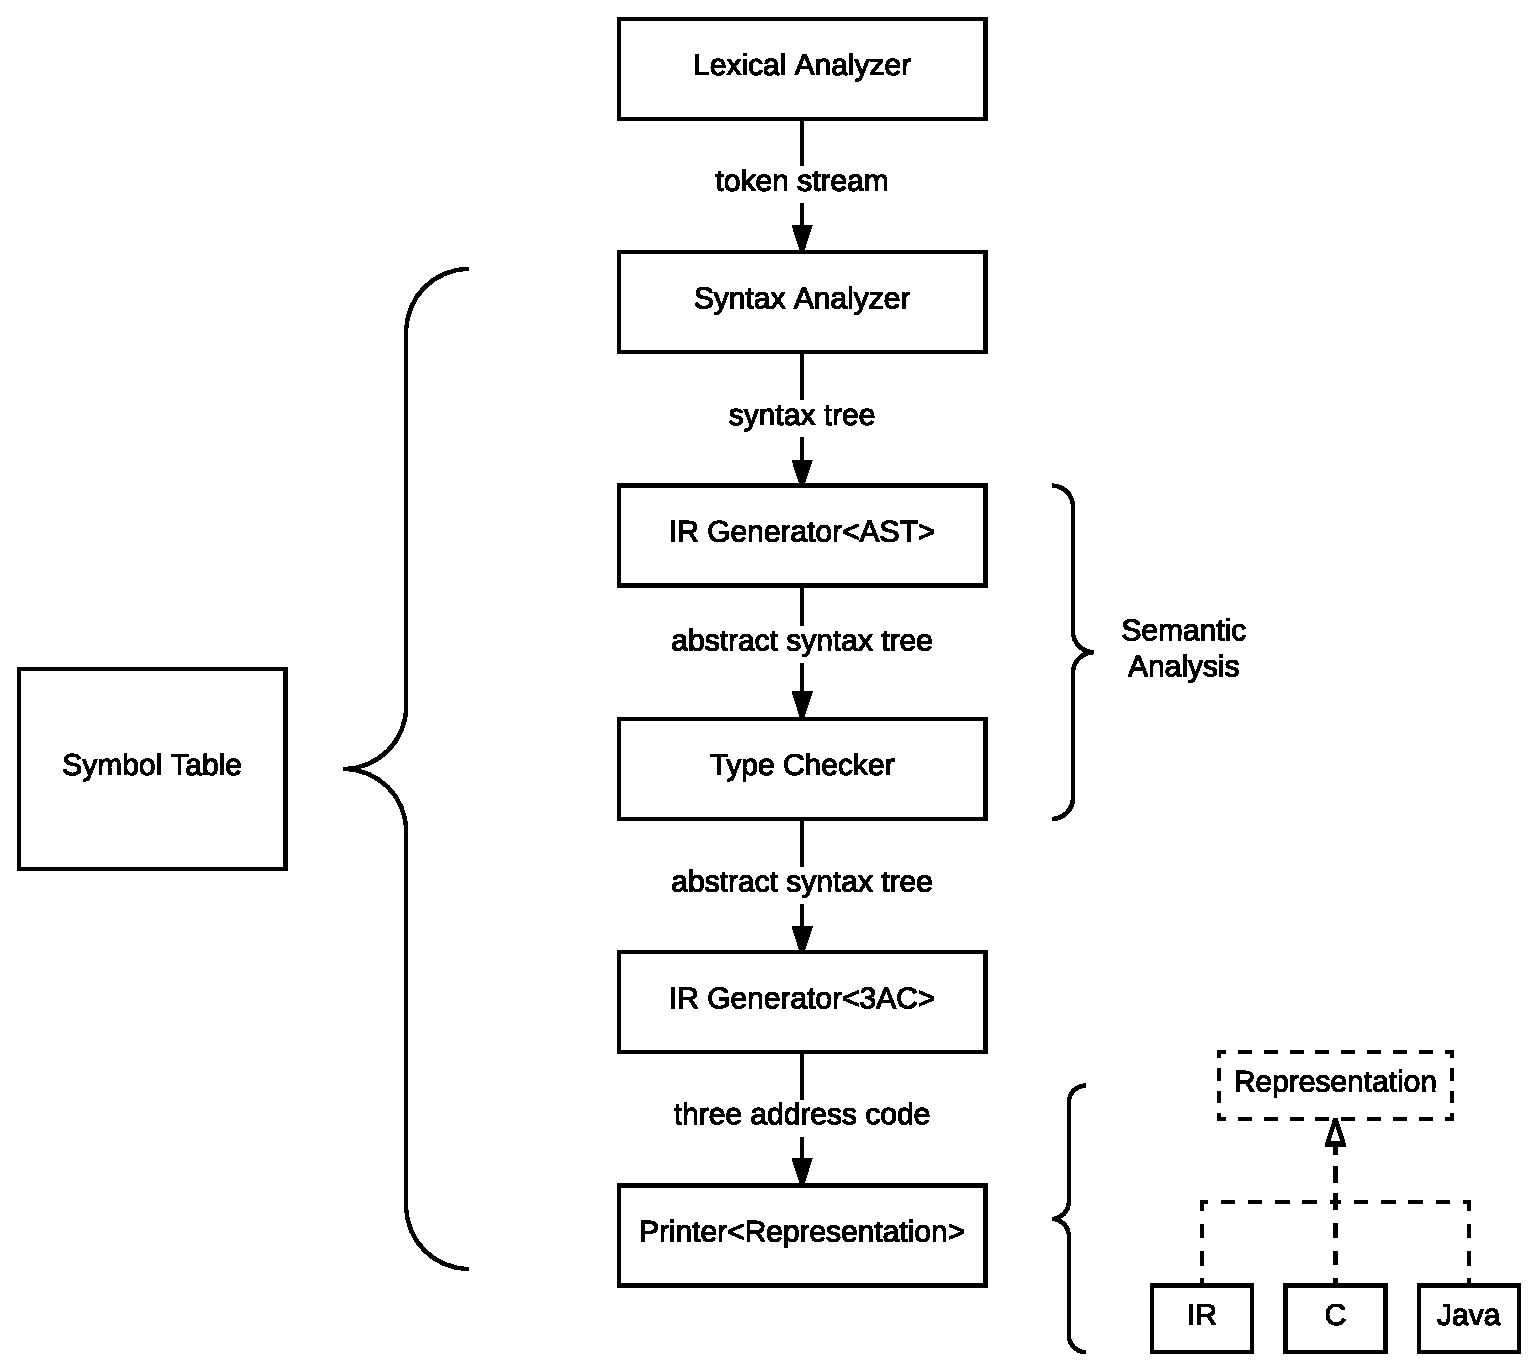
\includegraphics[width=.9\columnwidth]{img/eps/architecture.eps}
  \caption{Architectural Overview of the FAC compiler.}
  \label{fig:arch-ovw}
\end{figure}
